\section{The Development of the Mobile Client}
\subsection{Preconditions}
\label{subsec:Preconditions}
\subsubsection{Norms for Mobile Apps}
\label{subsubsec:Norms}
Because ePill is currently used in Germany only, we will focus on laws applicable in Germany. These laws are namely the \TKGns, the \TMGns, the \REG as well as the \DPA of \NRWns. The \TKG and \TMG are laws by state, whereas \REG is an european directive, specified by the respective Member States. 
\\
German federal states have their own \DPAsns. In this thesis we will focus on the \DPA of \NRW as ePill is located in \NRWns.
\\
\\
As the topmost layer of laws, the \REG defines more general directives. Article 4 defines national law applicable, if the natural or legal person, the controller\footnote{cf. \cite{TheEuropeanParliamentandtheCounciloftheEuropeanUnion.24.10.1995}, Article 2, (d)}, is located on a Member State's territory\footnote{cf. \cite{TheEuropeanParliamentandtheCounciloftheEuropeanUnion.24.10.1995}, Article 4, 1., (a) and (b)} or if any of the processing takes place on a Member State's territory\footnote{cf. \cite{TheEuropeanParliamentandtheCounciloftheEuropeanUnion.24.10.1995}, Article 4, 1., (c)}. It is required, that the controller asks the user to consent to the use and collection of data\footnote{cf. \cite{TheEuropeanParliamentandtheCounciloftheEuropeanUnion.24.10.1995}, Article 7, (a)}. Explicitly, "data concerning health and sex life"\footnote{\cite{TheEuropeanParliamentandtheCounciloftheEuropeanUnion.24.10.1995}, Article 8, 1.} shall not be processed, only if the user consent explicitly\footnote{cf. \cite{TheEuropeanParliamentandtheCounciloftheEuropeanUnion.24.10.1995}, Article 8, 2., (a)}, or if the processing is done by a healthcare professional under national law and for preventive medicine, medical diagnosis or treatment or for the management of health-care services\footnote{cf. \cite{TheEuropeanParliamentandtheCounciloftheEuropeanUnion.24.10.1995}, Article 8, 3.}. 
\\
\\
This is refined by the \TMGns. § 13 section (1) states, that the controller has to inform the user in a commonly understandable manner about the data which is collected and the form of processing of this data\footnote{cf. \cite{BundesregierungderBundesrepublikDeutschland.01.03.2007}, § 13, section (1)}. For a legal consent, the controller has to ensure, that the user is aware of his consent, that the consent is minuted, that the content of the consent is always available to the user and that the user can revoke his consent\footnote{cf. \cite{BundesregierungderBundesrepublikDeutschland.01.03.2007}, § 13, section (2)}.
\\
The same laws are stated in §§ 91, 93 and 94 of the \TKGns\footnote{cf. \cite{BundesregierungderBundesrepublikDeutschland.01.08.1996}, Section 2, §§ 91, 93, 94}.
\\
Also the \DPA of \NRW constitutes the same laws\footnote{cf. \cite{DerInnenministerdesLandesNordrheinWestfalen.09.06.2000}, Section 1, §§ 2, 4, 5} with the only restrictions, that its scope is limited to \NRWns.
\\
\\
Therefore ePill should explicitly inform the user that no data is stored and only anonymized transacted to find matching results, to comply with the stated laws.

\subsubsection{Best Practices}
\label{subsec:BestPractices}
The World Wide Web Consortium (W3C) has published a document in 2008 which states the basic best practices for developing for the mobile web. This document states 60 best practices, which shall ensure a minimum quality level for mobile web applications. These best practices emphasize the need of regard of the device's capabilities and supported technologies\footnote{cf. \cite{WorldWideWebConsortium.2008}, e.g. 2., 11., 21., 42.}. 
\\
The document focuses on mobile web development\footnote{cf. \cite{WorldWideWebConsortium.2008}, Abstract}, which has differences to native app development (e.g. the usage of frames and the accessibility of the device's specific features). Most of the best practices are applicable in both development environments.
\\
\\
For the mobile frontend of ePill, we can focus on best practices related to the user interface, input and navigation methods as well as general best practices, because it does not need more specific device capabilities, such as positioning and navigation features. Depending on the framework chosen, some of the best practices are already implemented by the framework. I.e. a thematic consistency\footnote{cf. \cite{WorldWideWebConsortium.2008}, 1.} is by default provided by frameworks such as TouchKit for Vaadin. Although they can be overridden, a consistent theme is provided. \cite{Wessels.2011} support the importance of a consistent appearance, cross platform and for both the mobile as well as the desktop application, if existent\footnote{cf. \cite{Wessels.2011}, p. 2}. \cite{Lica.2010} limits this to specific elements and points out, that mobile apps should provide just enough functionality to be useful and should not replicate the desktop optimized website.\footnote{cf. \cite{Lica.2010}, p. 66}
\\
Other best practices such as utilizing a navigation bar at the page's top\footnote{cf. \cite{WorldWideWebConsortium.2008}, 8.} for the main navigation are already adapted by different platforms and frameworks, such as Vaadin with TouchKit\footnote{cf. \url{https://vaadin.com/book/-/page/mobile.components.html}}, iOS\footnote{cf.\url{https://developer.apple.com/library/ios/documentation/UserExperience/Conceptual/MobileHIG/Navigation.html\#//apple_ref/doc/uid/TP40006556-CH53-SW1}} and Android\footnote{cf. \url{http://developer.android.com/design/get-started/ui-overview.html}}.
\\
\\
Best practices which are mainly determined by implementations of the developer, such as the usage of colors\footnote{cf. \cite{WorldWideWebConsortium.2008}, 26., 27} or the chosen input methods\footnote{cf.\cite{WorldWideWebConsortium.2008}, 55., 56., 57.} are often supported by the different platforms or frameworks but cannot be guaranteed by those. Even if different input methods such as a number pad for numeric inputs are provided by the framework or platform they still need to be adapted and utilized by the developer to act in line with the best practices.
\\
\\
The \cite{WorldWideWebConsortium.2008} furthermore specifies a "Default Delivery Context"\footnote{cf. \cite{WorldWideWebConsortium.2008}, 3.7 Default Delivery Context}, which defines the minimal capabilities for mobile devices which should be supported. \ref{tab:DefaultDeliveryContext} illustrates the minimal capabilities suggested by W3C.
\\
Nowadays it will be hard to match all of the requirements. E.g. a total maximum page weight of 20 kilobytes corresponds to the average file size of a 200 by 120 pixel JPEG-compressed file is about 10 kilobytes\footnote{Tested with 60\% compression rate and a random photograph} and two images would already exceed the maximum page weight. With mobile devices such as a Samsung Galaxy S3, which has a minimum of 720 pixel wide display, 120 pixels are far too less, even as a minimum width.
\\
Also nearly any mobile browser supports client side scripting (e.g. JavaScript). For more detail, \url{http://caniuse.com} holds compatibility charts of different browser features for nearly any browser available. The parsing of JavaScript Object Notation (JSON) for example is supported by 93.41\% of all mobile browsers according to caniuse\footnote{cf. \url{http://caniuse.com/\#cats=JS_API}, JSON parsing}.
\begin{table}[!tb]
    \center
    \begin{tabular}{l | p{21.5em}}
        \textbf{Parameter} & \textbf{Value} \\
        \hline
        Usable Screen Width & 120px \\
        \hline
        Markup Language Support & XHTML Basic 1.1 delivered with content type application/xhtml+xml. \\
        \hline
        Character Encoding & UTF-8 \\
        \hline
        Image Format Support & JPEG. \\
        & GIF 89a. \\
        \hline
        Maximum Total Page Weight & 20 kilobytes. \\
        \hline
        Colors & 256 Colors, minimum. \\
        \hline
        Style Sheet Support & CSS Level 1. In addition, CSS Level 2 @media rule together with the handheld and all media types. \\
        \hline
        HTTP & HTTP/1.0 or more recent. \\
        \hline
        Script & No support for client side scripting. \\
    \end{tabular}
    \caption[Mobile Default Delivery Context for Mobile Optimized Applications]{Default Delivery Context for Mobile Optimized Applications\footnotemark}
    \label{tab:DefaultDeliveryContext}
\end{table}
\footnotetext{cf. \cite{WorldWideWebConsortium.2008}, 3.7 Default Delivery Context}
\\
Nevertheless, minimizing the total page size is still a concern. \cite{Wessels.2011} points out, that smaller pages lead to faster load times and therefore provide a more efficient experience for the user.\footnote{cf. \cite{Wessels.2011}, p. 1066} \cite{Nicolaou.2013} suggests different approaches to reduce page size as well as load time: Scripts and markup should be minified\footnote{cf. \cite{Nicolaou.2013}, p. 49} and included inline\footnote{cf. \cite{Nicolaou.2013}, p. 50} where it is possible. Preloading components and reducing DNS lookups can also result in a faster user experience.\footnote{cf. \cite{Nicolaou.2013}, pp. 48, 49}
\\
Generally, \cite{Nicolaou.2013} recommend using a Content Delivery System (CDN), placing style sheets at the top of the source code, scripts at the bottom and using resized images rather than scaling them via HTML or CSS\footnote{cf. \cite{Nicolaou.2013}, pp. 49, 50}.
\\
\\
A study by \cite{Dahanayake.2010} came to the result, that 71\% of all responding web developers knew about the best practices, but only 11\% said, that they would understand these, 56\% have a vague understanding and 33\% do not understand the best practices.\footnote{cf. \cite{Dahanayake.2010}, p. 85}
\\
\\
\cite{AyobNurulZakiahbinti.2009} adjusted and combined four different guidelines for application development, namely Shneiderman’s Golden Rules of Interface Design, Seven Usability Guideline for Mobile Device (Abid Warsi, 2007), Human-Centred Design (ISO Standard 13407) and Mobile Web Best Practices 1.0 (W3C). Out of these guidelines, they developed the Three Layers Design Guideline for Mobile Application\footnote{cf. \cite{AyobNurulZakiahbinti.2009}, p. 430}. This guideline consists of three phases, which themselves represent different contexts, namely analysis (and the context of use), design (the context of medium) and testing (the context of evaluation). \ref{tab:ThreeLayersDesignGuideline} illustrates this guideline.
\\
\\
This thesis will follow the Three Layers Design Guideline, as it is the latest guideline and includes parameters set in a multitude of other guidelines. The third phase will be shortened due to the temporal restrictions of this thesis. The exact process will be outlined in the following subsections.

\begin{table}[!htb]
    \center
    \begin{tabular}{c | c | p{23.5em}}
        \multicolumn{2}{c | }{\textbf{Phase}} & \textbf{Context of Use and Activities} \\
        \hline
        1 & Analysis & \textbf{Use}: Specify user and organizational requirements \\
        \cline{3-3}
        & & 
            \begin{enumerate}
                \item Identify and document user’s tasks
                \item Identify and document organizational environment
                \item Define the use of the system
            \end{enumerate} 
        \\
        \hline
        2 & Design & \textbf{Medium}: Produce design solution \\
        \cline{3-3}
        & & 
            \begin{enumerate}
                \item Enable frequent users to use shortcuts
                \item Offer informative feedback
                \item Consistency
                \item Reversal of actions
                \item Error prevention and simple error handling
                \item Reduce short-term memory load
                \item Design for multiple and dynamic contexts
                \item Design for small devices
                \item Design for speed and recovery
                \item Design for “top-down” interaction
                \item Allow for personalization
                \item Don't repeat the navigation on every page
                \item Clearly distinguish selected items
            \end{enumerate}
        \\
        \hline
        3 & Testing & \textbf{Evaluation}: Evaluate design against user requirements \\
        \cline{3-3}
        & & 
            \begin{enumerate}
                \item Quick approach
                \item Usability testing
                \item Field studies
                \item Predictive evaluation
            \end{enumerate}
        \\
    \end{tabular}
    \caption[Three Layers Design Guideline for Mobile Application]{Three Layers Design Guideline for Mobile Application\footnotemark}
    \label{tab:ThreeLayersDesignGuideline}
\end{table}
\footnotetext{cf. \cite{AyobNurulZakiahbinti.2009}, p. 430, Table IV}

\subsubsection{Internal Requirements}
While developing a mobile frontend for ePill, it was important to us, that the main functionality of the web client will be optimized but not reduced in its main functionality. Therefore a good user interface is indispensable. All functionality should be accessible easily and without confusion for the user. Interactive elements such as buttons should be visible salient and have an immediate response to reduce the user's uncertainty.\footnote{cf. \cite{Norman2002}, p. 99} The general design, the color scheme and the fonts should be used in line with the web application to improve the recognition value.
\\
Another top priority is the accessibility of the app for as many users as possible. Therefore it is necessary to provide a cross-platform app that is accessible by as many mobile platforms as possible and to have an intuitive user interface which also enables elderly people to use it efficiently.
\\
\\
Modularity and flexibility is another important factor. ePill is designed to be flexible and scalable and the mobile client should incorporate the same idea. A scanning of barcodes on the packaging of pharmaceuticals could be implemented on a later stage to even further ease the use and increase the effectiveness.
\subsection{Analysis}
\label{subsec:Analysis}
\subsubsection{Assignment of a mHealth App Category}
The mobile app does not differ from the web application in terms of privacy risks, content or connectivity. The mobile app aims to provide the same main functionality as the web application optimized for mobile devices, therefore it also belongs to the same connectivity category, the medical connectivity, as the web application. Also no data is stored on the device and no additional usage data is sent to the server. 
\\
We plan to implement a SSL-encrypted connection to the server as soon as the later mentioned is capable of accepting and responding via SSL-encryption.
\\
\\
We would suggest to categorize the ePill mobile application as a low privacy risk, drug- and safety-related medical connectivity mHealth application and it should be categorized the same as the web application. 
\\
Possible future features might change the classification (e.g. the addressed barcode scanning) if data handling or storage is altered and with it other privacy risks may arise.

\subsubsection{The Different Operation Systems}
\paragraph{Android}$\;$

\vspace{0.75em}
Android is a mobile OS developed by the Open Handset Alliance\footnote{\url{http://www.openhandsetalliance.com}, last visited on 09/02/2013}, with Google being one of the biggest members. It is Linux based and was unveiled in 2007. Android is released by Google under the Apache License and is therefore Open Source.\footnote{cf. \url{http://source.android.com/source/licenses.html}, last visited on 09/02/2013} Developing for Android requires the Android SDK (or NDK) to be installed on the development computer. Developing apps with the SDK is done by writing Java code and defining the layout in specific XML\footnote{cf. for further details \url{http://developer.android.com}, last visited on 06/09/2013}. Android apps are executed in the Dalvik managed runtime\footnote{cf. \url{http://source.android.com/devices/tech/dalvik/index.html}, last visited on 09/09/2013} by default, except if they utilize the NDK. With the NDK apps can be (partly) written in C or C++ and are executed outside the Dalvik runtime which can be helpful for reusing existing code or executing CPU-intensive operations.\footnote{cf. \url{http://developer.android.com/tools/sdk/ndk/index.html}, last visited on 09/09/2013}
\\
\\
While Android is adapted by many manufacturers as well as consumers, a software-based and a hardware-based fragmentation is visible.\footnote{cf. for this and the next three following sentence \cite{DanHan.2012}, pp. 83, 92} Fragmentation means in this case a variety of different software and hardware which is at least partly incompatible. This fragmentation offers the user the choice to find exactly what he is looking for and enables more personalization. However, fragmentation may lead to non-consistent applications on different devices as well as delays in updates. According to Google, an Android version released 2010 (2.3 "Gingerbread") still has a distribution of around 30.7\%.\footnote{cf. \url{http://developer.android.com/about/dashboards/index.html}, last visited on 09/09/2013} This also implies that developers do not only have to regard latest versions of the OS, but also older versions. This means in return, that developers cannot always take full advantages of new capabilities as well as they need to pay much more attention to backwards compatibility.
\\
\\
For Android multiple IDEs are available. Eclipse\footnote{\url{http://www.eclipse.org}, last visited on 09/09/2013} is a popular IDE and is officially supported by the Android SDK.\footnote{cf. \url{http://developer.android.com/sdk/installing/bundle.html}, last visited on 09/22/2013} Android Studio, an Android optimized version of IntelliJ IDEA\footnote{\url{http://www.jetbrains.com/idea/}, last visited on 09/09/2013}, is still in development but already a stable IDE and greatly supported by Google\footnote{cf. \url{http://developer.android.com/sdk/installing/studio.html}, last visited 09/09/2013}.
\\
\\
Apps can be distributed directly to single phones or via an app store, e.g. the Google Play Store\footnote{\url{https://play.google.com/store}, last visited on 09/09/2013}. The Google Play Store has guidelines, which must be followed\footnote{\url{https://play.google.com/about/developer-content-policy.html}, last visited on 09/09/2013}, but no review process, in which compliance with the guidelines is verified, is performed.\footnote{for further information see \url{http://developer.android.com/distribute/googleplay/publish/preparing.html}, last visited on 09/24/2013}

\paragraph{iOS}$\;$

\vspace{0.75em}
iOS is the proprietary OS developed by Apple for mobile devices. It was first introduced in 2008. In contrast to the Android OS only Apple develops hardware and software that runs the iOS operation system. According to Apple, 94\% of all active iOS devices run the latest version of iOS 6.\footnote{cf. for this and the first following sentence \url{https://developer.apple.com/devcenter/ios/checklist/}, last visited on 09/11/2013} Compared to Android, all versions of iOS released before 2011 have a cumulative distribution of only 1\%. Hardware-based fragmentation on iOS is mainly based on the screen size: Two different for the phones and one for the tablets.
\\
\\
iOS apps can only be developed in Xcode\footnote{\url{https://developer.apple.com/xcode/}, last visited on 09/09/2013}, which is only available for Apple Mac. Xcode combines user interface design and coding. Coding is mainly done by writing Objective-C code but also supports native code written in C or C++. Designing interfaces is done with an Interface Builder called user interface integrated into Xcode.\footnote{cf. \url{https://developer.apple.com/library/ios/documentation/ToolsLanguages/Conceptual/Xcode_Overview/Edit_User_Interfaces/edit_user_interface.html\#//apple_ref/doc/uid/TP40010215-CH6-SW1}, last visited on 09/09/2013}
\\
\\
In contrast to Android, iOS apps can only be published via the Apple App Store\footnote{\url{http://appstore.com}, last visited on 09/11/2013}, or on registered devices with a special license by Apple\footnote{cf. \url{https://developer.apple.com/programs/ios/enterprise/}, last visited on 09/11/2013}. For submitting apps to the Apple App Store, one must obtain a developer license by Apple\footnote{cf. \url{https://developer.apple.com/programs/ios/}, last visited on 09/11/2013}. After submitting, all apps are reviewed and compared to Apple's guidelines\footnote{\url{https://developer.apple.com/appstore/guidelines.html}, last visited on 09/11/2013}.

\paragraph{Windows Phone 7 and 8}$\;$

\vspace{0.75em}
Windows Phone 7 was released in 2010 as the successor of Windows Mobile. Windows Phone 8, the phone version of Windows 8, were released in 2012. Both utilize the "Metro" design, a tile-based design.
\\
\\
Development for Windows Phone requires the Visual Studio IDE.\footnote{\url{http://www.microsoft.com/visualstudio/}, last visited on 09/11/2013} Visual Studio is only available for Windows. C\# or Visual Basic are the main programming languages and XAML is used for user interface design\footnote{cf. for this and the first following sentence \url{http://msdn.microsoft.com/en-US/library/windowsphone/develop/ff402529(v=vs.105).aspx}, last visited on 09/11/2013}. C++ can be utilized for graphic intensive applications.
\\
\\
The Windows Phone Store\footnote{\url{http://www.windowsphone.com/store}, last visited on 09/11/2013} is a closed store like the Apple App Store. This means, that an enrollment is needed to publish apps and the release of an app is preceded by a review process.\footnote{\url{http://msdn.microsoft.com/en-us/library/windowsphone/develop/hh184843(v=vs.105).aspx}, last visited on 09/11/2013} Unlike the other stores, the Windows Phone Store offers the possibility to try apps out with reduced functionality.

\paragraph{other}$\;$

\vspace{0.75em}
Depending on the source of statistics, the lead market share is held by different OS. Nevertheless other OS, e.g. Symbian, which was an important OS in 2008 with 47\% market share of smartphone OS\footnote{cf. "Canalys research release 2008/112" cited by \cite{Lin.2009}, p. 617, Figure 1}, is nowadays not listed at all or with less than 10\% market share\footnote{\url{http://gs.statcounter.com/\#mobile_os-ww-yearly-2008-2013}, last visited on 09/11/2013}\footnote{\url{http://www.idc.com/getdoc.jsp?containerId=prUS24257413}, last visited on 09/11/2013}\footnote{\url{http://blogs.strategyanalytics.com/WSS/post/2013/08/01/Strategy-Analytics-Android-Captures-Record-80-Percent-Share-of-Global-Smartphone-Shipments-in-Q2-2013.aspx}, Exhibit 1, last visited on 09/11/2013}.
\\
We will not take these OS into account, whose combined marketshare is around only 10\%, as this would exceed the time frame allocated for this thesis.

\subsubsection{Possible Frameworks and Technologies}
\paragraph{Completely native}$\;$

\vspace{0.75em}
Building native apps for supporting Android, iOS and Windows Phone, means maintaining three different projects in three different programming languages and three different user interface definitions. But native apps offer the most seamless user interface integration into the OS and the best performance. Native apps are developed for a specific OS and utilize the user interface controls provided by the OS. 
\\
While the seamless user interface integration could help people using the app in a familiar context, performance is not an issue for the ePill project. The costs for learning the specific aspects of those frameworks, developing and maintaining the three implementations are not reasonable for the given time frame of this thesis.
\\
\\
Additionally, we do not have an existing web service which the app could utilize to receive data from the server. With the logic already implemented, the currently used framework Vaadin does not offer a way to provide a web service. This additional effort is definitely a decisive argument.

\paragraph{HTML 5, jQuery mobile and Phone Gap}$\;$

\vspace{0.75em}
Providing an app for nearly any mobile device is possible with a web app. Based on web technologies like HTML, CSS and JavaScript, apps can be brought to nearly any mobile OS with only one implementation.
\\
As HTML5\footnote{\url{http://www.w3.org/TR/2012/WD-html51-20121217/}, last visited on 09/11/2013} and JavaScript is supported by most mobil devices, frameworks like jQuery mobile\footnote{\url{http://jquerymobile.com}, last visited on 09/11/2013} provide a common looking user interface without much additional effort. PhoneGap\footnote{\url{http://phonegap.com/}, last visited on 09/21/2013} enables web-based apps to access the device's capabilities like the camera or local storage. A detailed overview as well as unsupported features or OS can be found on PhoneGap's feature page\footnote{\url{http://phonegap.com/about/feature/}, last visited on 09/11/2013}.
\\
\\
Still, with this approach we would need a web service, which would be consumed with jQuery. The web app approach lessens the effort by developing multiple apps with only one code basis and user interface definition but still has the time consuming need for a new web service.

\paragraph{Xamarin}$\;$

\vspace{0.75em}
Xamarin\footnote{\url{http://xamarin.com}, last visited on 09/21/2013}, also known as MonoTouch, is an IDE and framework, which produces native apps for Android, iOS and Windows Phone from just a single C\# code basis. Different user interface definitions are still needed, but it combines the advantages of native apps and web apps. 
\\
Xamarin used with Visual Studio or Xamarin Studio, while Visual Studio is only available for Windows, Xamarin Studio is available for both Windows and Mac OS X.
\\
\\
Also apps developed with Xamarin would need an additional web service, which cannot be provided in the given time. Additionally, Xamarin is only free by meeting specific requirements, so it is likely to be more expensive than providing a web app.

\paragraph{Vaadin and TouchKit}$\;$

\vspace{0.75em}
Vaadin\footnote{\url{https://vaadin.com}, last visited on 09/11/2013} is a Java framework, with which the developer only needs to write application code and define a user interface included in the Java code. The framework builds the user interface as HTML and handles all communication between the client and the server. TouchKit\footnote{\url{https://vaadin.com/touchkit}, last visited on 09/11/2013} enables a Vaadin project to easily add a mobile web client. It provides various user interface controls which were optimized for mobile devices. It also provides access to the device's capabilities, such as positioning, offline storage or camera.
\\
\\
TouchKit supports iOS 5 or newer, Android 2.3 or newer and Windows Phone 8. Vaadin as well as it's add-on TouchKit, is focused on WebKit\footnote{\url{http://webkit.org}, last visited on 09/11/2013}-based browsers\footnote{cf. \url{https://vaadin.com/book/-/page/mobile.considerations.html}, last visited on 09/11/2013}, although it is compatible to most of the mobile browsers. Nevertheless, browsers which are not based on WebKit might be completely unusable or might have layout defects.
\\
\\
There are advantages to using Vaadin and TouchKit for ePill. More specifically, an additional web service is not necessary when using the existing code and simply adding a TouchKit-based user interface which seamlessly adapts to the existing code.

\subsubsection{The Choice for Vaadin and TouchKit}
Finally we chose Vaadin and the TouchKit add-on as the framework for the mobile frontend. The main reason to this is the lack of an accessible web service in Vaadin itself. Without a web service, we would have had to build a web service first to access the data layer or the application's logic.
\\
\\
Furthermore we wanted the complete system to be as homogenous as possible.  Utilizing the TouchKit Add-On for Vaadin, we reused as much existing code as possible and infrastructure by only adding another layer. This results in a much improved maintainability as the coding style is the same for the web application and the mobile application. Additionally no additional IDEs or frameworks need to be included or maintained.
\\
The missing compatibility to not WebKit-based browsers as well as the abstracted user interface definition might be drawbacks. With a less abstract user interface definition we would have more options to fine tune the resulting user interface.

\subsection{The Planning Process}
\label{subsec:Planning}
As already mentioned, the ePill system is already a functional prototype and the yet to develop mobile frontend is mostly an additional user-interface. Therefore no system-wide planning, including e.g. data organization, is needed but the data handling and user interfaces have to be planned.
\\
\\
Having the already existing application logic in mind, the planning of data handling is reduced to a functional planning\footnote{planning of the different functions available to the user and how they are accessed with which results and how error handling is performed}. To be able to have the functions available for the user, we have to combine the planning of the functional aspects with the user interface, therefore we will plan the user's flow through the application (user flow) which pays attention to the accessibility of the of the functions of the mobile web app in the right context during the use of the app, and combines functional and user interface planning. For the ease of explanation, we added some mockups and screenshots. We decided to show them uncolored to prevent distraction from highlighting colors and because the color scheme is not final yet. We decided to focus on smaller mobile devices such as phones and not on tablets, because smaller user interfaces can be expanded and are still usable. If the user interface is designed for a bigger screen and is presented on a smaller screen, either the elements become too small or the user needs to scroll through the interface. We will optimize the app's implementation for various layouts depending on the device's screen size at a later stage.
\\
\begin{figure}[ptbh]
    \begin{minipage}[b]{0.45\linewidth}
        \centering
        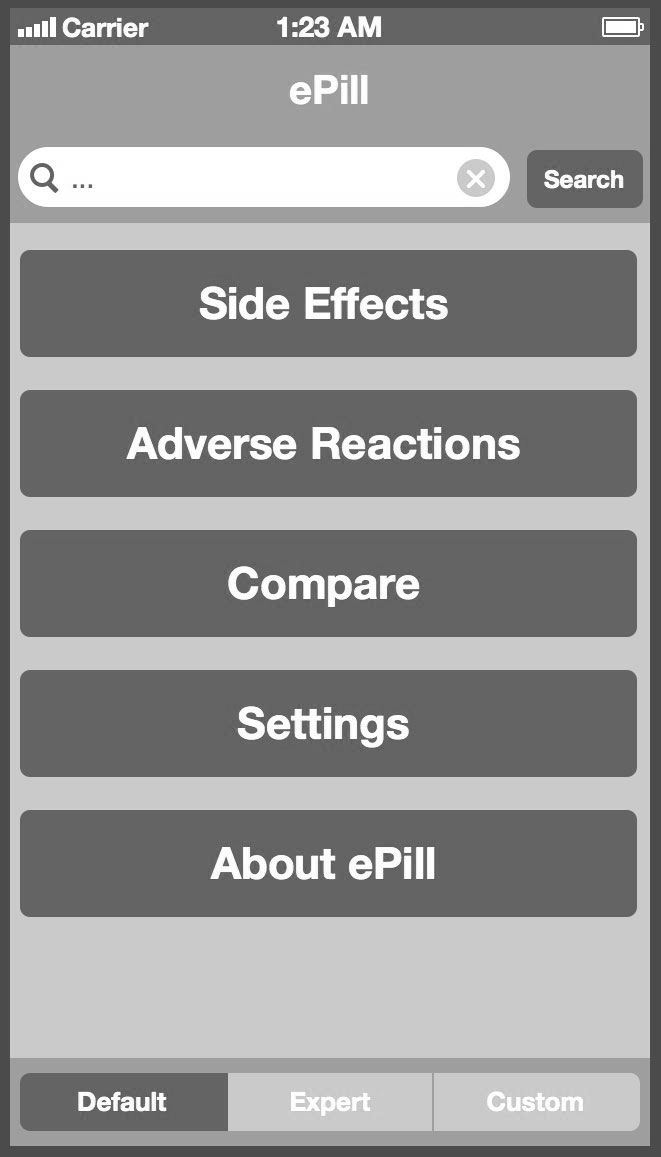
\includegraphics[width=0.8025\linewidth]{figures/Screen_1_bw.jpg}
        \caption[Main Screen Mockup]{Main Screen Mockup}
        \label{fig:Mockup}
    \end{minipage}
    \hspace{0.5cm}
    \begin{minipage}[b]{0.45\linewidth}
        \centering
        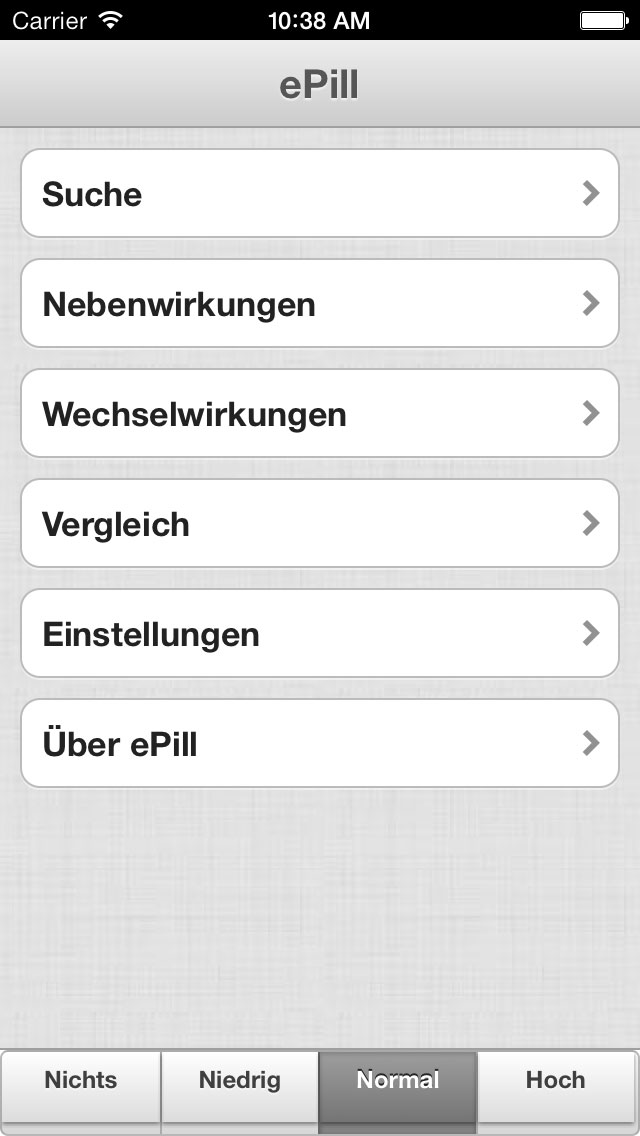
\includegraphics[width=0.8025\linewidth]{figures/Main_Screen_bw.jpg}
        \caption[Final Main Screen]{Final Main Screen}
        \label{fig:FinalMainScreen}
    \end{minipage}
    \\
    \\
    \\
    \begin{minipage}[b]{0.45\linewidth}
        \centering
        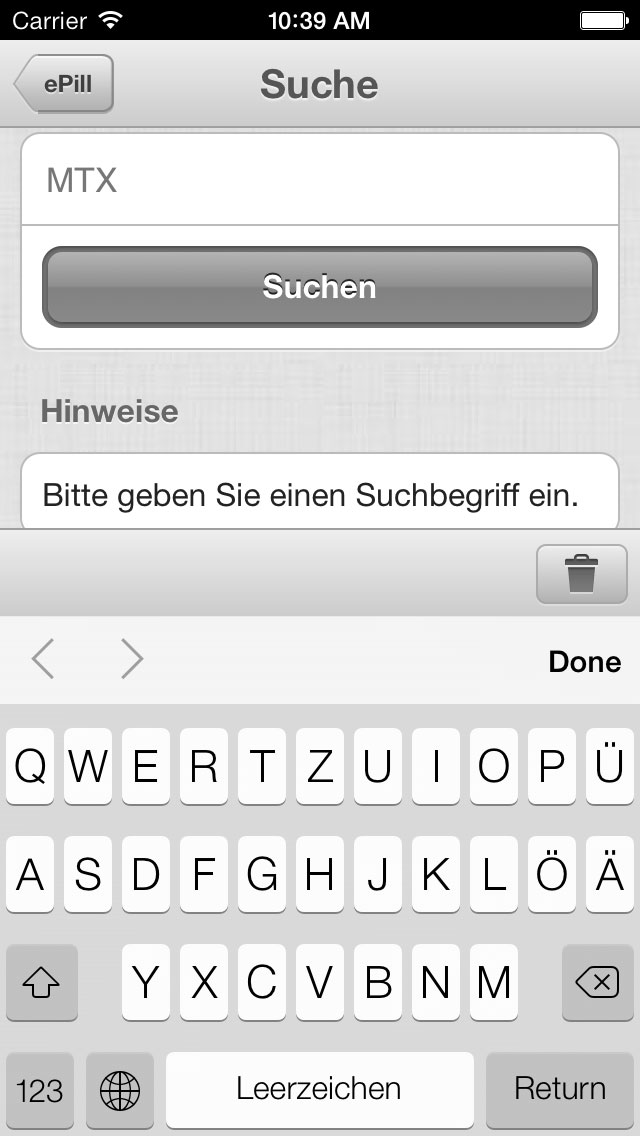
\includegraphics[width=0.8025\linewidth]{figures/Search_bw.jpg}
        \caption[Search Input Screen]{Search Input Screen}
        \label{fig:SearchInputScreen}
    \end{minipage}
    \hspace{0.5cm}
    \begin{minipage}[b]{0.45\linewidth}
        \centering
        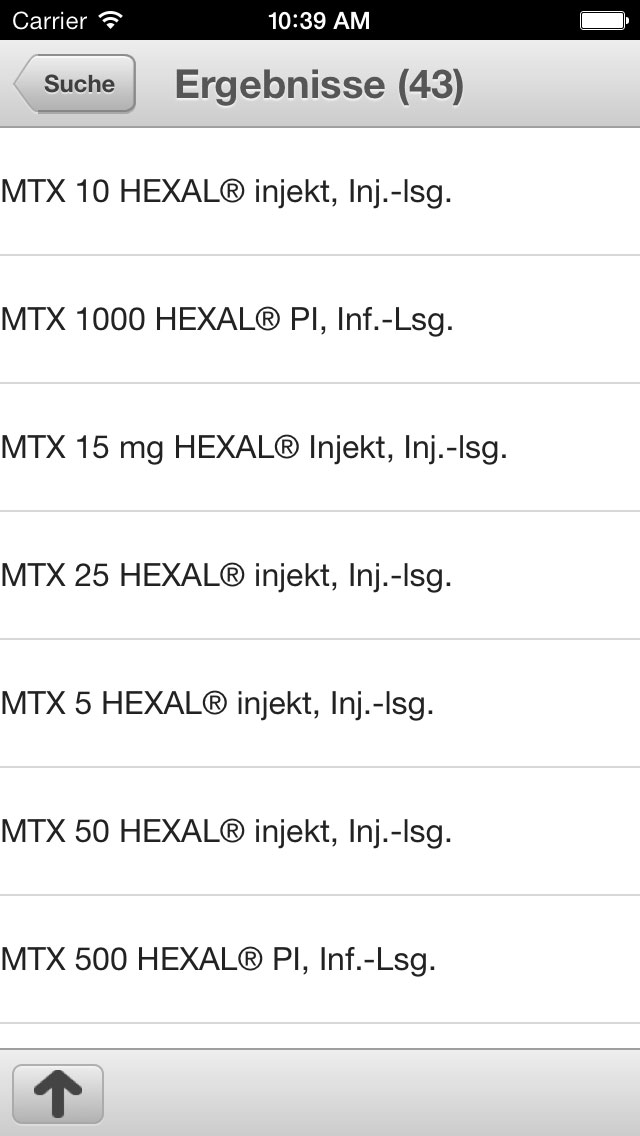
\includegraphics[width=0.8025\linewidth]{figures/Results_bw.jpg}
        \caption[Search Result Screen]{Search Result Screen}
        \label{fig:SearchResultScreen}
    \end{minipage}
\end{figure}
\\
The three major functions of ePill (Search, Display and Supplementing Services) should be accessible as fast as possible. The display functionality and some supplementing services (e.g. the term explanation functionality) are only able to present results if a pharmaceutical is selected. So we designed \ref{fig:Mockup} as a minimal starting screen with every main function quickly accessible. Due to some missing user interface controls provided by Vaadin TouchKit, such as the search bar, we finally implemented the start screen as illustrated in \ref{fig:FinalMainScreen}. This furthermore resulted in a more separated presentation of search string input view and result view, as presented in \ref{fig:SearchInputScreen} and \ref{fig:SearchResultScreen}.
\\
\\
Throughout the planning and designing we tried to reproduce common patterns and user interface controls, that are well know through the usage of other apps, and therefore we utilized the navigation back button on the top left corner, which is illustrated by a leftwards oriented arrow-shaped button. Central navigation which specifies the view is centered in the main content area at the center of the screen.
\\
\\
Most of the views offer a toolbar at the bottom of the screen. This toolbar contains controls which are used for navigation inside the view at the center of the screen, such as the ability to go back, to the top or to navigate to a specific headline. In the pharmaceutical details view with all the information visible, it can be very handy to jump right to the header one is interested in. Additionally, some controls are added in the toolbar which enable further interaction with the information displayed, e.g. adding the currently visible pharmaceutical to the comparison list, which we will discuss soon.
\\
\\
The web application has rich customization possibilities. One can adjust the font size, the details of pharmaceuticals to be displayed and the layout of the web application itself. As it turned out, it is not applicable for the user to change the mobile apps layout, because the user interface so too compact to add additional elements and too few elements are visible to deem it necessary to hide any given element.
\\
\\
The comparison list is a concept added to the mobile application and derived from an element in the web application. The web application provides a view in which pharmaceuticals can be added and afterwards, via a button click, be compared. Aggregated information such as adverse reactions can also be listed. Because we have much less available screen space in the mobile app, we decided to keep the list globally available throughout the entire app. For example, if one searched for a pharmaceutical and has selected one to display detailed information, he can easily add this pharmaceutical (via a button in the toolbar) to his comparison list. If one now selects the "side effects" functionality on the main screen, he sees his comparison list and can add addition pharmaceuticals to it. This screen is illustrated in \ref{fig:CurrentListScreen}. One is now presented a search input screen but can in the search result screen only tick on those pharmaceuticals he wants to add to his comparison list, which is illustrated in \ref{fig:AlternativeListScreen}.
\\
\begin{figure}[!b]
    \begin{minipage}[b]{0.45\linewidth}
        \centering
        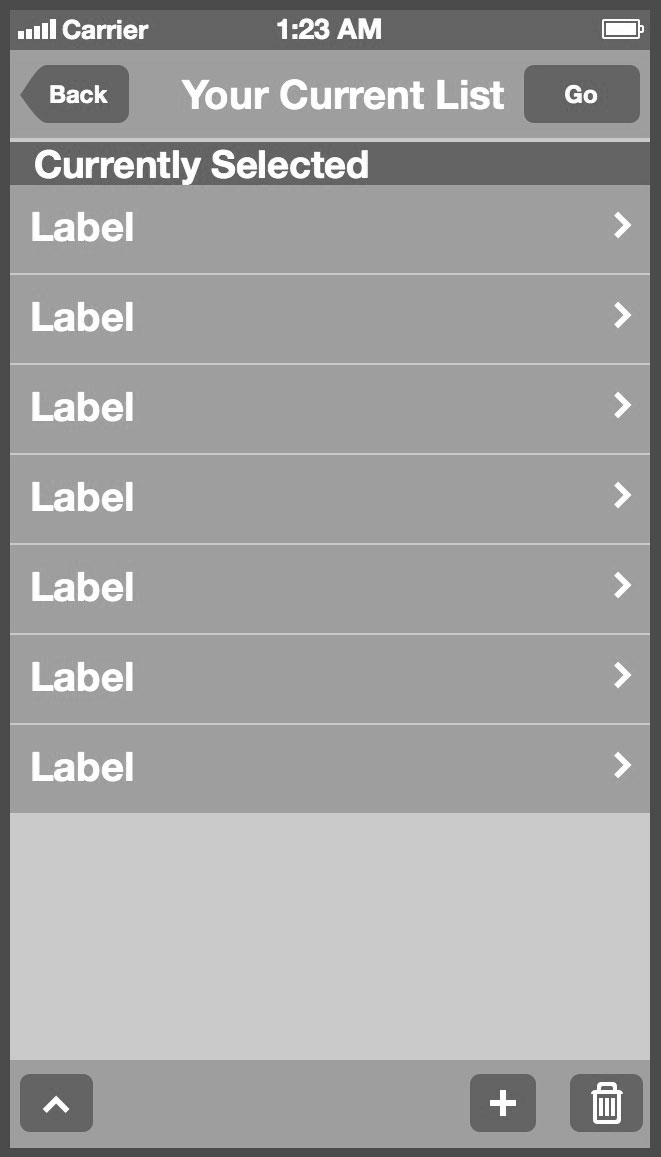
\includegraphics[width=0.8025\linewidth]{figures/Screen_2_bw.jpg}
        \caption[Comparison List Screen Mockup]{Comparison List Mockup}
        \label{fig:CurrentListScreen}
    \end{minipage}
    \hspace{0.5cm}
    \begin{minipage}[b]{0.45\linewidth}
        \centering
        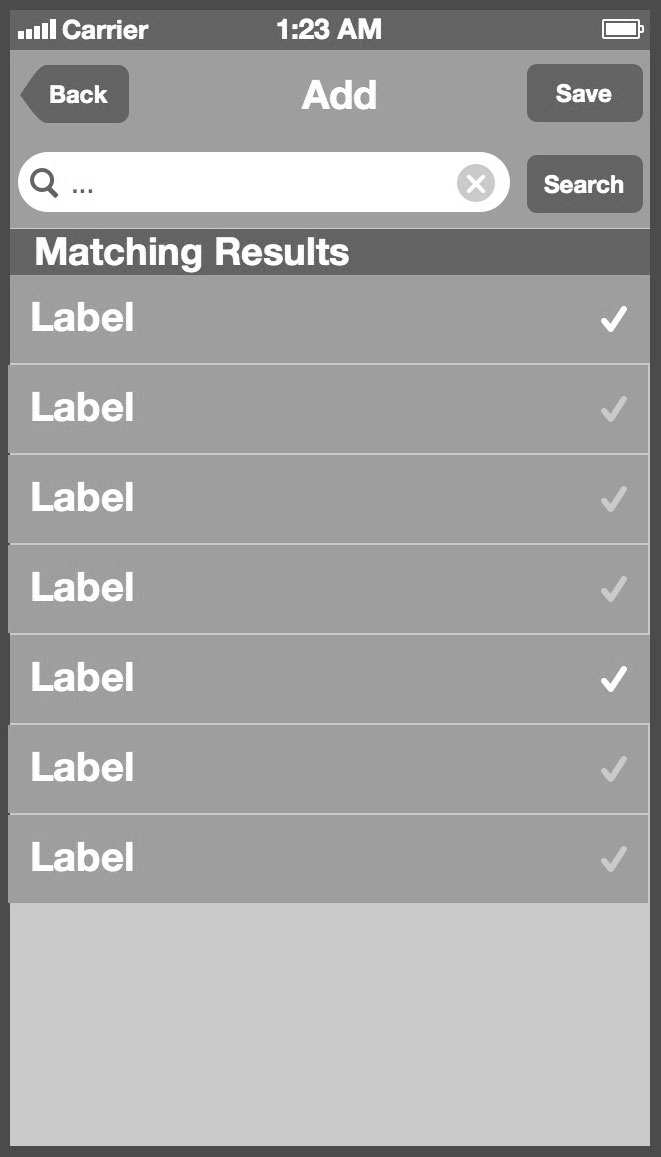
\includegraphics[width=0.8025\linewidth]{figures/Screen_3_bw.jpg}
        \caption[List Screen to add to Comparison List Mockup]{Results Screen Mockup}
        \label{fig:AlternativeListScreen}
    \end{minipage}
    \\
    \\
    \\
    \begin{minipage}[b]{0.45\linewidth}
        \centering
        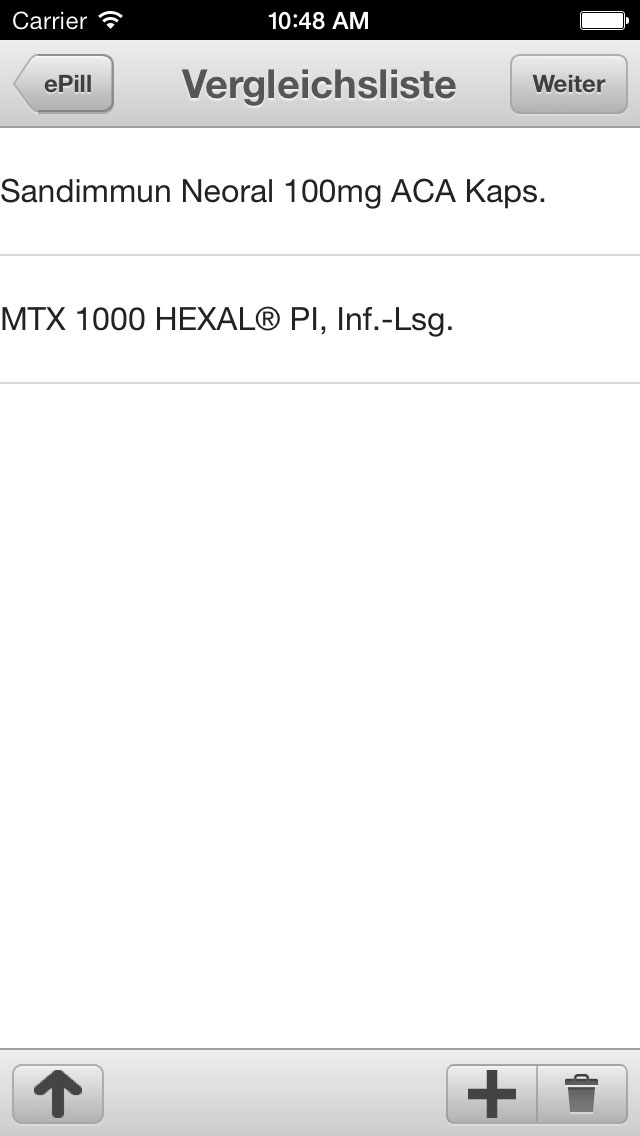
\includegraphics[width=0.8025\linewidth]{figures/List_bw.jpg}
        \caption[Comparison List Screen]{Comparison List Screen}
        \label{fig:CurrentListScreen}
    \end{minipage}
    \hspace{0.5cm}
    \begin{minipage}[b]{0.45\linewidth}
        \centering
        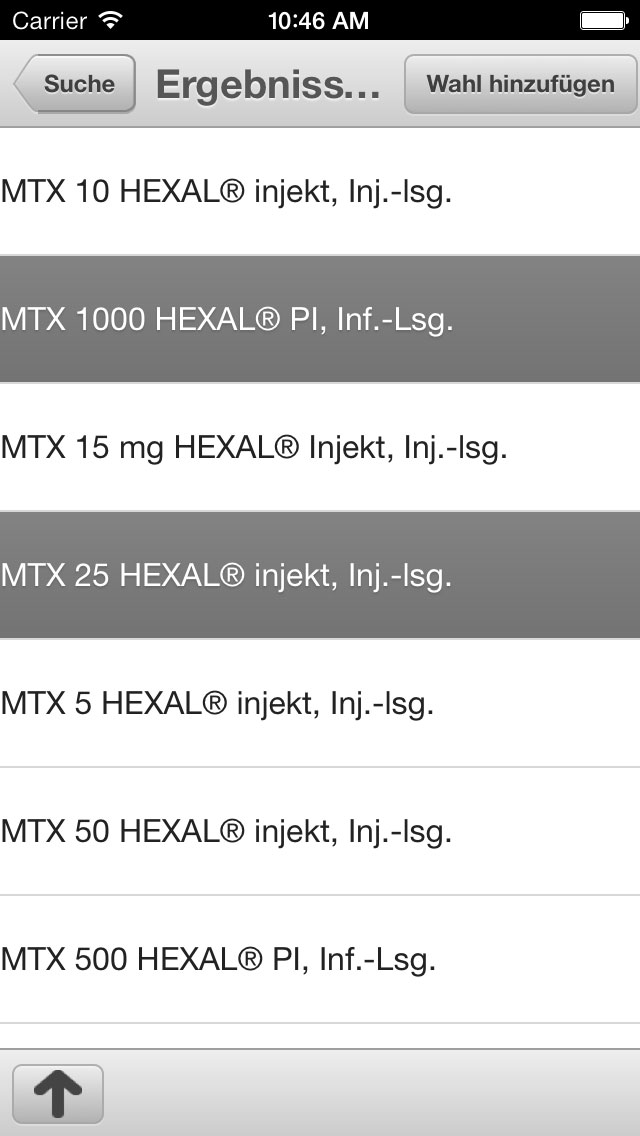
\includegraphics[width=0.8025\linewidth]{figures/Results_Alt_bw.jpg}
        \caption[List Screen to add to Comparison List]{Results Screen}
        \label{fig:AlternativeListScreen}
    \end{minipage}
\end{figure}
\\
\begin{figure}[ptb]
    \begin{minipage}[b]{0.45\linewidth}
        \centering
        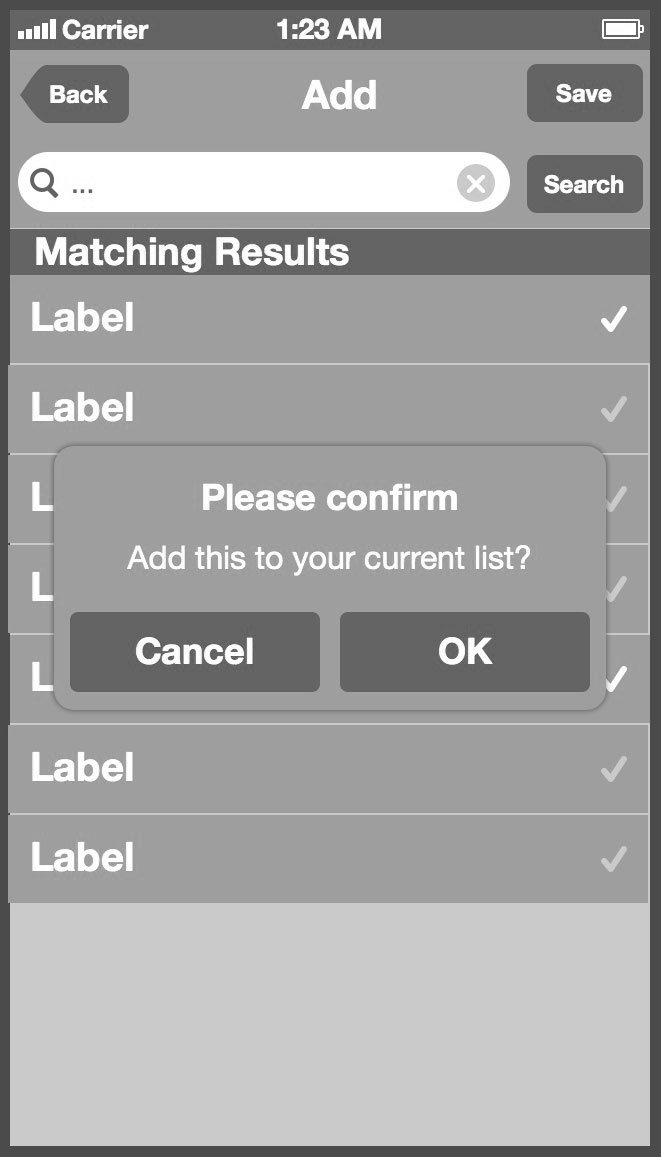
\includegraphics[width=0.8025\linewidth]{figures/Screen_3a_bw.jpg}
        \caption[Confirm Action Dialog]{Confirm Dialog Mockup}
        \label{fig:ConfirmDialog}
    \end{minipage}
    \hspace{0.5cm}
    \begin{minipage}[b]{0.45\linewidth}
        \centering
        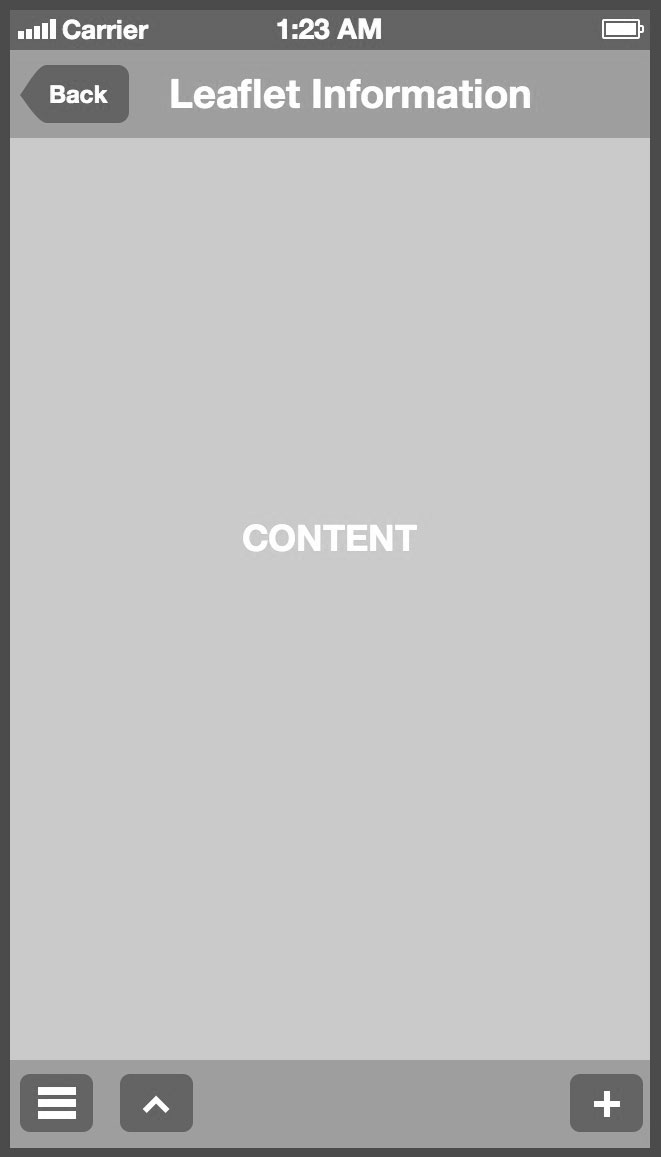
\includegraphics[width=0.8025\linewidth]{figures/Screen_4_bw.jpg}
        \caption[Pharmaceutical Details Screen]{Details Screen Mockup}
        \label{fig:DetailsScreen}
    \end{minipage}
    \\
    \\
    \\
    \begin{minipage}[b]{0.45\linewidth}
        \centering
        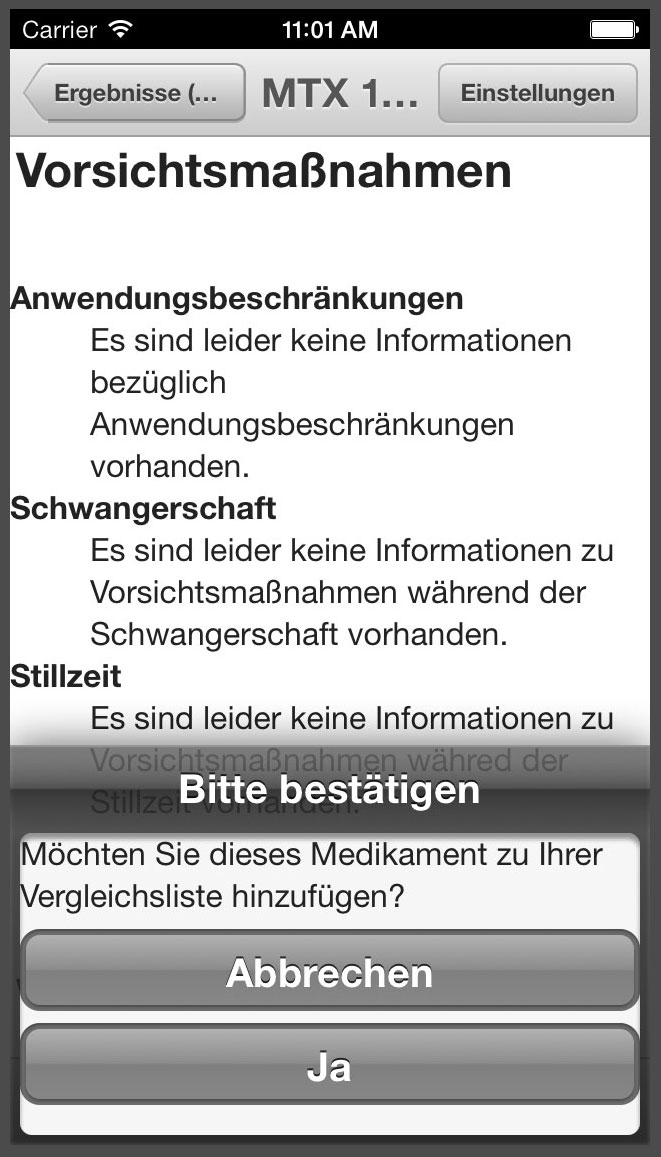
\includegraphics[width=0.8025\linewidth]{figures/Dialog_bw.jpg}
        \caption[Confirm Action Dialog]{Confirm Dialog}
        \label{fig:ConfirmDialog}
    \end{minipage}
    \hspace{0.5cm}
    \begin{minipage}[b]{0.45\linewidth}
        \centering
        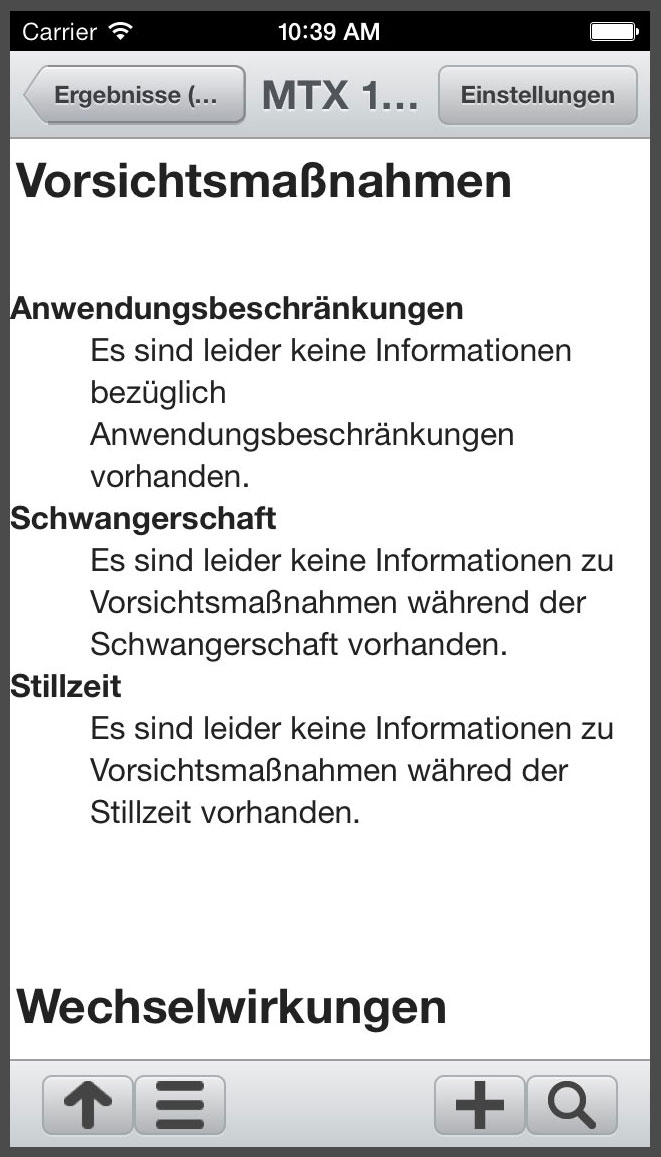
\includegraphics[width=0.8025\linewidth]{figures/Detail_bw.jpg}
        \caption[Pharmaceutical Details Screen]{Details Screen}
        \label{fig:DetailsScreen}
    \end{minipage}
\end{figure}
\\
\ref{fig:CurrentListScreen} also highlights the toolbar. The leftmost button scrolls back to the top, whereas on the right side we have an add button which brings up the already discussed search view and the trash button, which clears the comparison list. 
\\
The button on the top right corner, labeled "Go", starts the currently selected function, e.g. adverse reactions on the comparison list.
\\
To prevent users from misusage, we will add dialogs asking to confirm the chosen operation where adequate. This currently only effects the delete and add operations of the comparison list, as illustrated in \ref{fig:ConfirmDialog}.
\\
\ref{fig:DetailsScreen} illustrates the pharmaceuticals details screen. This screen presents all information for a specific pharmaceutical, e.g. after the selection of one pharmaceutical in the search results screen or from the comparison list as illustrated in \ref{fig:CurrentListScreen}. Basically, this screen consists of the back navigation button in the top left corner, the toolbar in the bottom and the centered main content area as most of the mobile app's screens. While the main content area displays the chosen leaflet information in a segmented way, the toolbar offers different operations. On the lower right corner, the add button allows the user to add the currently selected pharmaceutical to his comparison list. The left side of the toolbar offers a back to top button just such as the comparison list screen as well as a navigation button, enabling the user to jump to any of the sections by which the main content is segmented. A click on this button reveals a list of the sections through which the user can scroll and select one to navigate to. Another click on this button closes the list as well as the section selection.

\subsection{The Implementation Process}
\label{subsec:Implementation}
We had some issues at the beginning of the implementation of the planned user flow, because Vaadin and TouchKit differ to other frameworks we worked with beforehand. For instance, TouchKit does not provide a search bar which can be attached to the navigation bar as planned in the mockups, furthermore the ePill web application is currently written in Vaadin 6, whereas TouchKit 3 is based on Vaadin 7. We tried to utilize Vaadin 6 and TouchKit 2 for the mobile app but as it turned out, TouchKit 2 has some drawbacks in comparison to TouchKit 3, such as a smaller documentation, tutorials and example projects. The choice for Vaadin 7 and TouchKit 3 resulted in, that we could not just include the ePill web application and directly access the business logic, as adjustments were needed to upgrade a Vaadin 6 project. 
\\
We decided to include as much as possible from the web application and copy and modify as little as possible. During further development, after the web application was upgraded to Vaadin 7, both projects could be merged together and code redundancies can be removed. The choice for Vaadin 7 brought additional work as we had to adjust inner code references to e.g. the main window and application because their handling did change.
%\\
%\\
%After having set the stage for the implementation, we discovered that Vaadin does not seem to have a community as big and as active as Node.js\footnote{\url{http://nodejs.org}} or django\footnote{\url{https://djangoproject.com}}. While we made the experience that to most issues an answer can be found in the related forums, mailing lists or community pages as well as on more general websites such as Stack Overflow\footnote{\url{http://stackoverflow.com}}, only very few answers and questions were found on Stack Overflow regarding Vaadin or TouchKit. A direct comparison between the official django mailing list\footnote{\url{https://groups.google.com/forum/\#!forum/django-users}} and the Vaadin forum\footnote{\url{http://vaadin.com/forum}} revealed that while the django mailing list had 40,367 topics\footnote{last visited on 09/16/2013}, the Vaadin forum had 14,523 threads\footnote{last visited on 09/16/2013}, including news and forum guidelines. Nevertheless, the Vaadin forum was often helpful.
\\
\\
Programming with Vaadin is easy after the first steps into the framework were successful. The coding style supposed by the framework was consistent and helped achieving fast results. Nevertheless, missing controls are a drawback and the inflexibility of the framework is both an advantage and disadvantage. While the given user interface controls and the limited influence on their exact appearance help providing a consistent user interface, they prevent from optimizing and fine tuning. For instance, it is not easily possible to access device specific functionality by utilizing APIs of the specific OS. PhoneGap can be integrated but this also means addition effort for utilizing an additional framework.
\\
\\
The lack of components such as alert- and confirm-dialogs or search bars is compensable. During the development, we utilized popovers to imitate the well known appearance of dialogs in most of the mobile OS. Vaadins popover component is functional, as it provides an overlay with a responsive layout\footnote{a layout which adjusts to the screen size} for different screen sizes but is not completely customizable. For instance, the bar at the popovers top cannot be customized and buttons cannot be added to this bar. Vaadins popover has also a much bigger border than we would have used with a common dialog component. This reduces the useable content area. Additionally the borders distract the user and reduces the focus on the content and buttons.
\\
\\
We implemented a workaround for the missing search bar attached to the navigation bar by adding an additional view. As stated beforehand, we planed to attach the search bar directly beneath the navigation bar to enable the user to quickly access the search functionality. Results were planned to be displayed as an overlay list. We had to abandon the idea of an overlay list as well. Overlays looked either unfamiliar or complicated the use of the app, especially for dismissing the results. Finally we chose to display a view containing an input field, a search button and a label displaying information such as the minimum length of the query. The results are displayed in another standalone view as a plain list.
\\
\\
Another issue we discovered was the drop for dynamic style sheets and themes in Vaadin 7. In Vaadin 6 one could swap the used theme during runtime, which would be useful to adjust the font size. In the allocated time frame, we were not able to implement a workaround. We tried adjusting the font size dynamically by adding CSS classes to the different user interface controls but this either resulted in a high complexity for the algorithm to discover all matching controls nor high memory usage if we were to keep references for the controls.
\\
\\
Thanks to the automatic handling of references between the client- and the server-side, E.g. the settings screen for customizing the displayed leaflet information could be implemented quickly. Nevertheless it was not possible to receive specific events such as a "will appear" or "did appear" for views, which are called either if the user navigates to this screen or is navigated backwards to this screen. These events are needed for refreshing the view or specific controls if needed. Java and Vaadin offer listeners for "value changed" events but those still need a reference to the controls, which need to be passed along through the views. The main screen contains a toolbar at the screens bottom to select a preset of visible information on leaflets. If the user decides to change the preset in a lower view, this toolbar needs to be updated as well. Additionally to the increased reference count this method has the drawback that the toolbar gets updated on every value change, although it is not visible. With a "will appear" event the update would have been done only once immediately before the toolbar becomes visible.
\\
\\
Parts of the layout from the web application could be reused with only minor adjustments, thanks to Vaadins seamless TouchKit integration. We had to make adjustments on the layout of tables, especially the count of columns as well as the preloaded content. We reduced the displayed information to a minimum for usability but comprehensibility. Comparing two pharmaceuticals can only be effective, if related information is presented closely. During the development we experimented with a vertical instead a horizontal layout, meaning that each related information of the two pharmaceuticals are presented beneath each other, not side by side, but it became very confusing because of the doubled page length. With the headlines beneath each other, one needed to scroll too much to compare the pharmaceuticals directly. We concluded that a horizontal layout and a landscape orientation will be best in this case. The landscape orientation provided enough screen space on most devices to have associated headlines side by side which eased the comparison.

\subsection{Validation of the Mobile App}
\label{subsec:Validation}
In this section we will compare the developed app to the norms and best practices highlighted in section \ref{subsec:Preconditions} \nameref{subsec:Preconditions}, as well as to all requirements stated in section \ref{subsec:Analysis} \nameref{subsec:Analysis}.
\\
\\
Because no user-related data is stored, neither personal nor usage related, no conflicts with the norms mentioned in section \ref{subsubsec:Norms} \nameref{subsubsec:Norms} were discovered.
\\
\\
Vaadin and TouchKit support developers by providing a default theme for applications to maintain a consistent user interface, design and color wise. Despite the statement of \cite{Wessels.2011} that a consistency to a desktop application should be maintained\footnote{cf. \cite{Wessels.2011}, p. 1067}, we focused on an easy to use user interface on mobile devices. Some parts look very familiar on both applications, e.g. the detailed informations or the comparison of pharmaceuticals, but the navigation is absolutely different as a result of the limited screen size and a touch- instead of mouse-based operation. This differentiation was chosen with the statement of \cite{Lica.2010} in mind that the mobile app should only provide enough functionality to be useful\footnote{cf. \cite{Lica.2010}, p. 66}. This resulted likewise in a missing customizable tab-bar or different sidebars. These elements might be operational on a bigger screened device such as tablets, but it is not useable on most mobile phones. Further development of the mobile app might result in an optimized tablet user interface and integrate this functionality.
\\
In sections \ref{subsec:Planning} \nameref{subsec:Planning} and \ref{subsec:Implementation} \nameref{subsec:Implementation} we stated that we utilized a navigation bar and a toolbar as main interaction controls for navigation and direct interaction such as clearing lists. These two concepts of placing controls on the edges of the screen are also recommended by \cite{WorldWideWebConsortium.2008}.\footnote{cf. \cite{WorldWideWebConsortium.2008}, 8.}
\\
We also tried to follow common input methods. As no specific input fields for e.g. numbers, were needed, the only specialization we could use was the enter-key equivalent on mobile devices, often a button on the lower right corner of the simulated on-screen keyboard.
\\
The \cite{WorldWideWebConsortium.2008} suggested a "Default Delivery Context"\footnote{cf. \cite{WorldHealthOrganization.2011}, 3.7 Default Delivery Context} illustrated in \ref{tab:DefaultDeliveryContext} \nameref{tab:DefaultDeliveryContext}, but Vaadin does not leave much to the developer to optimize the rendering of the controls as well as the organization of requests and client-side handling of data. Developers can only optimize used images and CSS style sheets. Because only very few images are used and not much custom styling is applied, we could not pursue this recommendation in particular.
\\
\\
Comparing this app to the Three Layers Design Guideline developed by \cite{AyobNurulZakiahbinti.2009}, illustrated in \ref{tab:ThreeLayersDesignGuideline}, results in the following: While phase one, the analysis, was already done by \cite{Dehling.2012}, phase two was one of the purposes of this thesis.\footnote{cf. for this and the following paragraph \cite{AyobNurulZakiahbinti.2009}, p.430, Table IV} We tried to implement shortcuts where possible with the help of toolbars and quick access to settings, specially in the detail view, and offered informative feedback where possible, e.g. for the search right beneath the input field or in popovers for detailed information. Using the same theme and general user interface layout led to the proposed consistency as well as the optimization for small devices. The utilization of a navigation bar at the top also compiles with the proposed "top-down" interaction or navigation. Vaadin as the framework as well as the already existing code support error prevention and handling through catching thrown exceptions and giving a direct response to the user. Personalization is made possible with the settings view which enables the user to select only those information to be displayed he is interested in. \cite{Norman2002} states, that grouping controls into logical and functional modules as well as hiding infrequently used controls is a good way to reduce complexity.\footnote{cf. \cite{Norman2002}, p. 175, 6.9} We grouped the main functions as buttons onto the main screen, added a toolbar at the bottom for quick access to the detail level settings and hid all functionality on another screen, accessible via the mentioned buttons.
\\
Phase three, testing, could only be done superficially until the end of this thesis' time frame. We did only a short functional testing. Further development might pursue a more detailed testing of the mobile app.
\\
\\
The internal requirements were compiled with, buttons were made salient and interaction with them resulted in immediate feedback. For instance, the search button disables itself until the server processed the request hence the user cannot execute the search twice. The mobile app is available on nearly any mobile platform because of the good distribution of HTML 5 compatible browsers. Also, the app is as modular as the web application because much code was reused and only adapted to the changes in Vaadin 7 compared to Vaadin 6 and the layout was optimized for small screens. The color scheme used by the web application was not adapted because of the more general familiarity among mobile OS users with the TouchKit default theme because of its similarity to the appearance of iOS apps as well as other mobile web apps.
\\
\\
We propose that further development might improve the utilized default TouchKit theme, for a more effective and intuitive use of the mobile app. We would set the focus on the popovers which are currently not matching perfectly to the overall appearance. Nevertheless, the mobile app follows the guidelines stated in section \ref{subsec:Preconditions} \nameref{subsec:Preconditions} and should provide a good user interface and functionality. A dedicated usability test may reveal some remaining weak points.